% contributors: Nihaar Shah
\section{Poincar\'e Embeddings for Hierarchical Representations}
We start by discussing \cite{Poincar\'e}. In this paper, the authors introduce a new approach for learning hierarchical representations of symbolic data by embedding them into hyperbolic space and more specifically into an n-dimensional Poincare ball. The motivation for this is to capture latent hierarchical structure in complex symbolic datasets which is often lost by merely embedding into a Euclidean vector space. The efficient algorithm introduced here to learn the embeddings empirically shows superior performance than Euclidean ones both in terms of the representation capacity as well as generalization ability. 
\\ Generally, similarity between objects in the embedding space is measured primarily in terms of their distance and/or inner product (hence their orientation). Here we consider the distances as a measure. 
\subsection{Preliminaries}
\subsubsection{Hyperbolic space}
Hyperbolic space is a space exhibiting Hyperbolic geometry. The primary difference from Euclidean geometry is that the parallel axiom of Euclidean geometry (i.e. parallel lines do not intersect) doesn't hold in Hyperbolic geometry while the remaining axioms do hold.
\begin{figure}
    \centering
    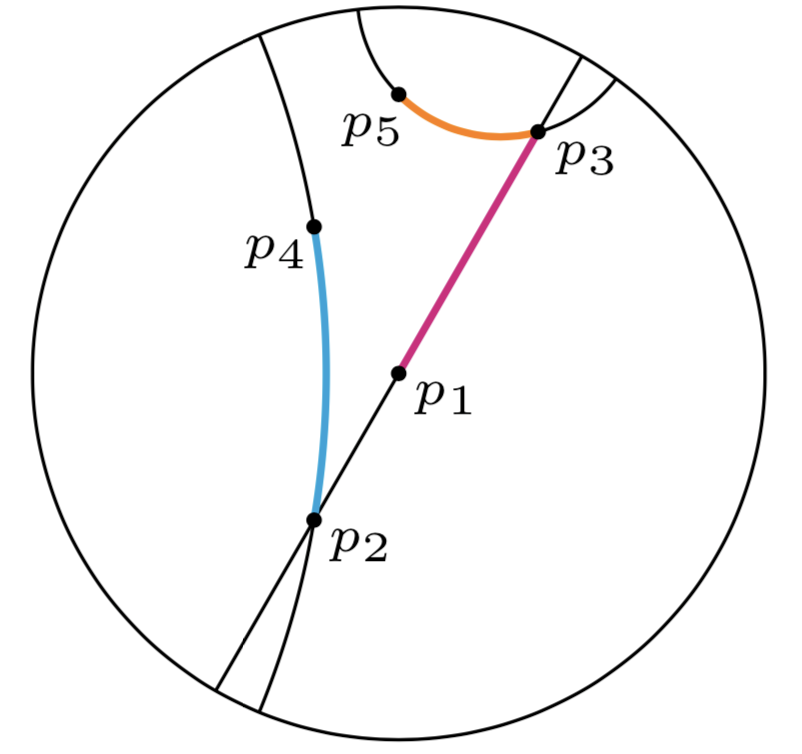
\includegraphics[width=.4\textwidth]{chapter_16/files/poincare1.png}
    \caption{Geodesics of a Poincare disk. Note the hyperbolic disk area and the circle length grow exponentially the closer they are to the boundary. }
    \label{hyperb-tree}
\end{figure}
Informally, hyperbolic space can be thought of as a continuous version of trees and a space with constant negative curvature. This relationship between hyperbolic space and a tree can be visualised by considering the growth rate of branches (b) of a tree as the level (l) of the tree progresses. For a branching factor b a tree has $$(b+1)b^{l-1}$$ nodes at level 'l' while $$((b+1)b^l-2)/(b-1)$$ nodes on a level $\leq l$. The number of children grows exponentially with distance from the root. In hyperbolic geometry, this relation can be modeled naturally because the disc area and circle length grow exponentially with radius (as compared to the Euclidean distance). Consider the 2 dimensional hyperbolic space with constant curvature $K=-1$ where the length of a circle is $$2 \pi \text{sinh} r = 2 \pi ((e^r - e^{-r})-1)$$ and the disc area is $$2 \pi (cosh r -1) =2 \pi ((e^r + e^{-r})-1)$$. Thus both disc area and the circle length grow exponentially with r (relative to their euclidean distance) as also illustrated in fig \ref{hyperb-tree}.
\subsubsection{Poincare Embeddings}
Particularly, the model of hyperbolic space being considered is a Poincare ball model because it lends itself to gradient based Riemann optimization ( shall be discussed) which is easily parallelizable.
\\This paper wishes to reflect the latent hierarchy in which symbols can be organized in the embedding space in two ways:
\begin{itemize}
    \item Inducing an appropriate bias on the structure 
    \item Capturing the hierarchy explicitly in the embedding space to gain insights about the relationships between symbols and the importance of individual symbols.
\end{itemize}
Crucially, the information about hierarchy e.g. ordered input pairs is not directly accessible and hence the task of inferring these relationships in a fully unsupervised way is tackled by embedding the symbolic data into Hyperbolic space $\mathbb{H}$.
\bigskip
\\Let us define an open d-dimensional unit ball where $\norm{.}$ is th Euclidean norm 
$$\mathbb{B}^d = \{\mathbf{x} \in R^d | \norm{\mathbf{x}}<1\}$$
The Poincare ball model of hyperbolic space corresponds then to the Riemannian manifold $(\mathbb{B}^d,g_x)$ which is the open unit ball with Riemannian metric tensor\footnote[1]{A metric tensor is a type of function which takes as input a pair of tangent vectors v and w at a point of a surface and produces a real number scalar g(v, w).  A manifold equipped with a positive-definite $(g(v, v) > 0$ to every nonzero vector v) metric tensor is known as a Riemannian manifold.}:
$$g_x = (\frac{2}{1 - \norm{\mathbf{x}}^2})^2 g^E$$
Here $\mathbf{x} \in B^d$ and $g^E$ denotes the Euclidean metric tensor. The distance between points $\mathbf{u,v}\in \mathbb{B}^d$ is:
\begin{equation}
    d(\mathbf{u,v}) = \text{arcosh }(1+ \frac{2 \norm{\mathbf{u - v}}^2}{(1 - \norm{\mathbf{u}}^2)(1 - \norm{\mathbf{v}}^2)})\label{dist-poin}
\end{equation}
The above equation \ref{dist-poin} crucially shows that the distance within the Poincare ball changes smoothly with respect to location $\mathbf{u}$ and $\mathbf{v}$ - a locality property which will be key to finding continuous embeddings of hierarchies.
\subsection{Optimization}
Let:
$$\mathbb{T}_\theta \mathbb{B} \text{ - denote the tangent space of a point} \mathbf{\theta} \in B^d$$ 

$$\nabla_R \in \mathbb{T}_\theta \mathbb{B} \text{ -denote the Riemannian gradient of } \mathbb{L}(\theta)$$

$$\nabla_E \text{ denote the Euclidean gradient of } \mathbb{L}(\theta)$$ 
Riemannian adaptive Optimization Methods (RSGD) parameter updates are of the form:
\begin{equation}
    \theta_{t+1} = R_{\theta_t}(-\eta_t \nabla_R \mathbb{L}(\theta_t))
\end{equation}
Where $R_{\theta_t}$ denotes the retraction\footnote[2]{retraction is a continuous mapping from a topological space into a subspace that preserves the position of all points in that subspace} onto $\mathbb{B}$ at $\theta$. To derive the Riemann gradient from the Euclidean gradient, it is sufficient to re-scale $\nabla_E$ with the inverse of the Poincare ball metric tensor $g_\theta^{-1}$. In particular, the Euclidean gradient is:
\begin{equation}
    \nabla_E = \frac{\partial \mathbb{L}(\theta)}{\partial d(\theta,x)}\frac{\partial d(\theta,x)}{\partial \theta}
\end{equation}
which we see is dependent on the gradient of $\mathbb{L}$ which we assume is known. The partial derivatives of the Poincare distance can be computed as follows: Let $\alpha = 1 - \norm{\theta}^2$, $\beta = 1-\norm{x}^2$ and let:
\begin{equation}
    \gamma = 1 + \frac{2}{\alpha \beta }\norm{\theta - x}^2
\end{equation}
Then the partial derivative of the Poincare distance with respect to $\theta$ is:
\begin{equation}
    \frac{\partial d(\theta,x)}{\partial \theta} = \frac{4}{\beta \sqrt{\gamma^2 -1}}(\frac{\norm{x}^2 -2\langle \theta , x \rangle +1}{\alpha^2}\theta - \frac{x}{\alpha}) \label{poincare-diff}
\end{equation}
We constrain the embeddings to remain within the Poincare ball via the projection:
\begin{equation}
\text{proj}(\theta)
    \begin{cases}
        \theta / \norm{\theta} - \epsilon &\text{if  }\norm{\theta} \geq 1 \\ 
        \theta & \text{  otherwise  }
    \end{cases}
\end{equation}
In summary, the full update for a single embedding is then:
\begin{equation}
    \theta_{t+1} \leftarrow \text{ proj }(\theta_t - \eta_t \frac{(1- \norm{\theta_t}^2)^2}{4}\nabla_E) \label{summary-eq} 
\end{equation}
As we have seen, this optimization algorithm has related the Euclidean gradient to Riemann gradient. Furthermore, equations \ref{poincare-diff} and \ref{summary-eq} reveal the highly parallelizable nature of gradient updates making this framework feasible.
\subsection{Discussion of evaluation tasks and metrics}
It is worth noting some applications (here within Natural Language Processing) for which this framework and the evaluation metrics used. Note the type of distance function used besides the Euclidean $\norm{u -v}^2$ is called Translational distance $\norm{u-v+r}^2$ which is valuable for asymmetric data where the global translational vector $r$ is also learned during training. They use transitive closure of the WORDNET noun hierarchy in the following two settings.
\subsubsection{Embedding of taxonomies}
The hypernymy \footnote{semantic association of being a part of a higher class for e.g. bir is the hypernymy of eagle,pigeon,crow etc.} relations form a directed acyclic graph such that the hierarchical structure is not directly visible from the raw data but has to be inferred. Also note that negative samples are created by randomly picking 10 pairs per positive sample for which there is no relation or link in the tree. The loss used to learn such an embedding is the following.
$$L(\Phi) = \Sigma_{(u,v)\in D} log (\frac{e^{-d(u,v)}}{e^{-d(u,v')}})$$
This choice of loss function is because we don’t want to push symbols belonging to distinct subtrees arbitrarily far apart as their subtrees might still be close. Instead we want them to be farther apart than symbols with an observed relation. Fig \ref{poincare-embedding} shows the hypernymy relations for the reconstructed subtree of the word "Mammals". It is worth noting the greatly improved performance of Poincare embeddings over Translational embeddings (note we mentioned the Translational distance metric previously).
\begin{figure}
    \centering
    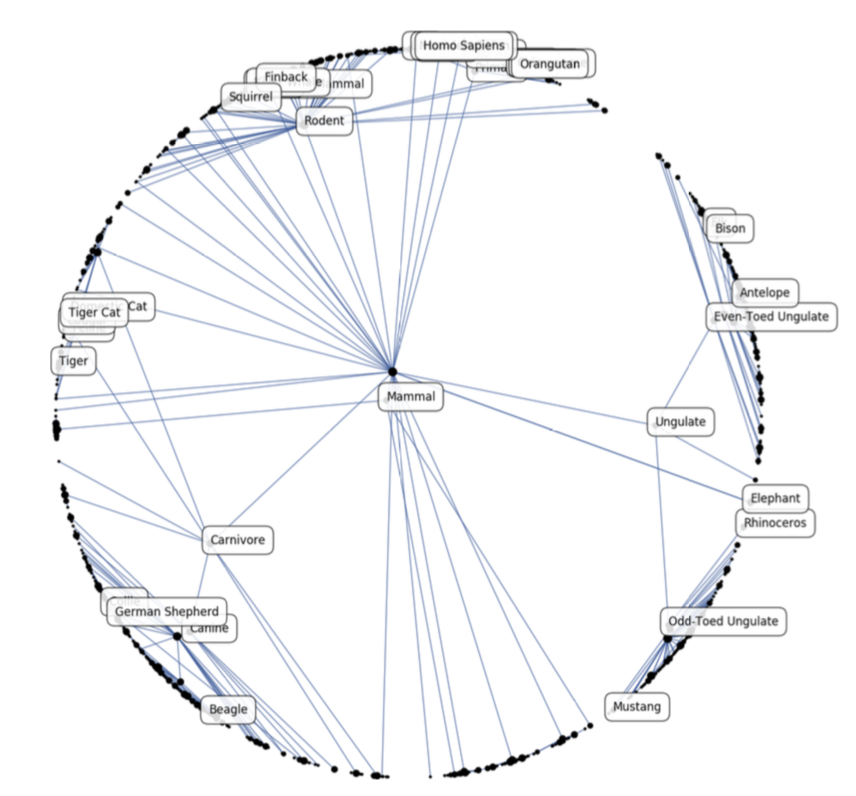
\includegraphics[width=.7\textwidth]{chapter_16/files/poincare-embedding.png}
    \caption{Caption}
    \label{poincare-embedding}
\end{figure}
The measures of efficacy for embeddings of taxonomies are 1) reconstruction of words from embeddings (measured in Mean Average Precision of the ranking of all nouns) 2) link predictions by randomly holding out links.
\subsubsection{Network Embeddings}
This is also a task of link prediction in networks but in social networks datasets.  The probability of an edge is modelsed as Fermi-Dirac distribution:
$$P((u,v) = 1 | \Phi)= \frac{1}{e^{(d(u,v)-r)/t}+1}$$
Here, r corresponds to the radius around each point u such that points within this radius are likely to have an edge with u. The parameter t specifies the steepness of the logistic function and influences both average clustering as well as the degree distribution. It can be seen that Poincar\'e embeddings perform again very well on these datasets and – especially in the low-dimensional regime – outperform Euclidean embeddings.
\subsection{Conclusion}
In this paper, they introduced Poincare embeddings for learning representations of symbolic data and showed that they can learn similarity and hierarchy of objects. They introduced a highly parallelizable algorithm for learning that was based on Riemannian optimization. Finally this setup was evaluated on two tasks: learning taxonomies of embeddings of words and link prediction in social network graphs. Poincare embeddings showed promise in both settings. 
